% fig_network_attack_protect: the attack-protect (firefighter-type) game on a
% small tree.  The leader attacks at most 2 nodes, then the follower protects
% at most 2; fire spreads from attacked nodes through unprotected neighbours;
% the follower maximises the saved nodes, the leader minimises them.
% Tree (15 nodes): r - {a, b, c}; a - {a1, a2}; a1 - a11; b - {b1, b2, b3};
% b2 - {b21, b22}; c - {c1, c2}; c1 - c11.
% Checked by enumeration of every attack (<= 2 nodes) and every protection
% (<= 2 nodes): the bilevel optimum is 8 saved.  Shown: attack {a, b} (optimal),
% the follower's best answer protects {r, b2}; burnt: a1 a11 a2 b1 b3;
% saved: r b2 b21 b22 c c1 c2 c11 (8 of 15).
% Build: pdflatex fig_network_attack_protect.tex   (3.15 in x 1.8 in)
\documentclass[tikz,border=2pt]{standalone}
\usepackage{mathptmx}
\usetikzlibrary{arrows.meta,calc}
\definecolor{leader}{HTML}{2A78D6}
\definecolor{follower}{HTML}{EB6834}
\definecolor{cert}{HTML}{1BAF7A}
\definecolor{ink}{HTML}{0B0B0B}
\definecolor{ink2}{HTML}{52514E}
\definecolor{muted}{HTML}{A9A8A2}
\definecolor{grid}{HTML}{E6E5E0}
\definecolor{critical}{HTML}{D03B3B}
\tikzset{
  every picture/.style={font=\fontsize{8}{9.6}\selectfont, color=ink, line cap=round, line join=round},
  small/.style={font=\fontsize{7}{8.4}\selectfont},
  tedge/.style={ink2, line width=0.6pt},
  fire/.style={critical!70, line width=1.3pt},
  % node glyphs (radius 0.17 cm)
  pics/attacked/.style={code={
    \fill[critical] (0,0) circle (0.19);
    \fill[white] (0.035,0.15) .. controls (0.02,0.09) and (0.115,0.05) .. (0.095,-0.035)
      .. controls (0.08,-0.115) and (-0.08,-0.115) .. (-0.095,-0.035)
      .. controls (-0.105,0.025) and (-0.07,0.05) .. (-0.055,0.085)
      .. controls (-0.04,0.05) and (-0.02,0.04) .. (-0.005,0.045)
      .. controls (0.0,0.08) and (0.02,0.11) .. cycle;
    \fill[critical] (0.005,0.035) .. controls (0.01,0.0) and (0.05,-0.02) .. (0.04,-0.055)
      .. controls (0.03,-0.085) and (-0.03,-0.085) .. (-0.04,-0.055)
      .. controls (-0.05,-0.025) and (-0.01,-0.005) .. cycle;}},
  pics/burnt/.style={code={
    \draw[critical, line width=0.8pt, fill=critical!22] (0,0) circle (0.15);}},
  pics/protected/.style={code={
    \draw[follower!80!black, line width=0.6pt, fill=follower]
      (-0.155,0.16) -- (0.155,0.16) -- (0.155,0.02)
      .. controls (0.155,-0.09) and (0.06,-0.15) .. (0,-0.20)
      .. controls (-0.06,-0.15) and (-0.155,-0.09) .. (-0.155,0.02) -- cycle;}},
  pics/saved/.style={code={
    \draw[ink2, line width=0.7pt, fill=white] (0,0) circle (0.15);}},
}
\begin{document}
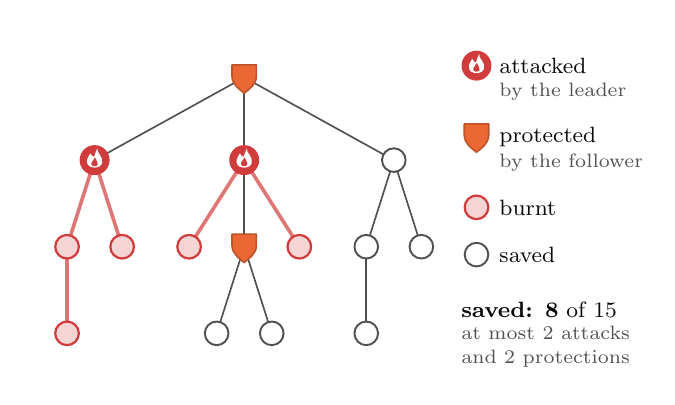
\begin{tikzpicture}
  % fixed page: 3.15 in x 1.8 in including the 2 pt border
  \useasboundingbox (0,0) rectangle (7.86,4.432);

  % node positions
  \coordinate (r)   at (2.75,3.8);
  \coordinate (a)   at (0.85,2.75);  \coordinate (b)   at (2.75,2.75);  \coordinate (c)   at (4.65,2.75);
  \coordinate (a1)  at (0.50,1.65);  \coordinate (a2)  at (1.20,1.65);
  \coordinate (b1)  at (2.05,1.65);  \coordinate (b2)  at (2.75,1.65);  \coordinate (b3)  at (3.45,1.65);
  \coordinate (c1)  at (4.30,1.65);  \coordinate (c2)  at (5.00,1.65);
  \coordinate (a11) at (0.50,0.55);
  \coordinate (b21) at (2.40,0.55);  \coordinate (b22) at (3.10,0.55);
  \coordinate (c11) at (4.30,0.55);

  % edges: the fire's path in red, the rest grey
  \foreach \u/\v in {r/a, r/b, r/c, b/b2, b2/b21, b2/b22, c/c1, c/c2, c1/c11}
    \draw[tedge] (\u) -- (\v);
  \foreach \u/\v in {a/a1, a/a2, a1/a11, b/b1, b/b3}
    \draw[fire] (\u) -- (\v);

  % nodes
  \foreach \n in {a, b} \pic at (\n) {attacked};
  \foreach \n in {a1, a2, a11, b1, b3} \pic at (\n) {burnt};
  \foreach \n in {r, b2} \pic at (\n) {protected};
  \foreach \n in {b21, b22, c, c1, c2, c11} \pic at (\n) {saved};

  % key
  \begin{scope}[shift={(5.5,0)}]
    \pic at (0.2,3.95) {attacked};
    \node[anchor=west, inner sep=1pt] at (0.45,3.95) {attacked};
    \node[small, anchor=west, inner sep=1pt, text=ink2] at (0.45,3.62) {by the leader};
    \pic at (0.2,3.05) {protected};
    \node[anchor=west, inner sep=1pt] at (0.45,3.05) {protected};
    \node[small, anchor=west, inner sep=1pt, text=ink2] at (0.45,2.72) {by the follower};
    \pic at (0.2,2.15) {burnt};
    \node[anchor=west, inner sep=1pt] at (0.45,2.15) {burnt};
    \pic at (0.2,1.55) {saved};
    \node[anchor=west, inner sep=1pt] at (0.45,1.55) {saved};
    \node[anchor=west, inner sep=0pt, align=left] at (0.0,0.85)
      {\textbf{saved: 8} of 15};
    \node[small, anchor=west, inner sep=0pt, align=left, text=ink2] at (0.0,0.38)
      {at most 2 attacks\\ and 2 protections};
  \end{scope}
\end{tikzpicture}
\end{document}
